

\begin{figure}[htbp]
    \centering
    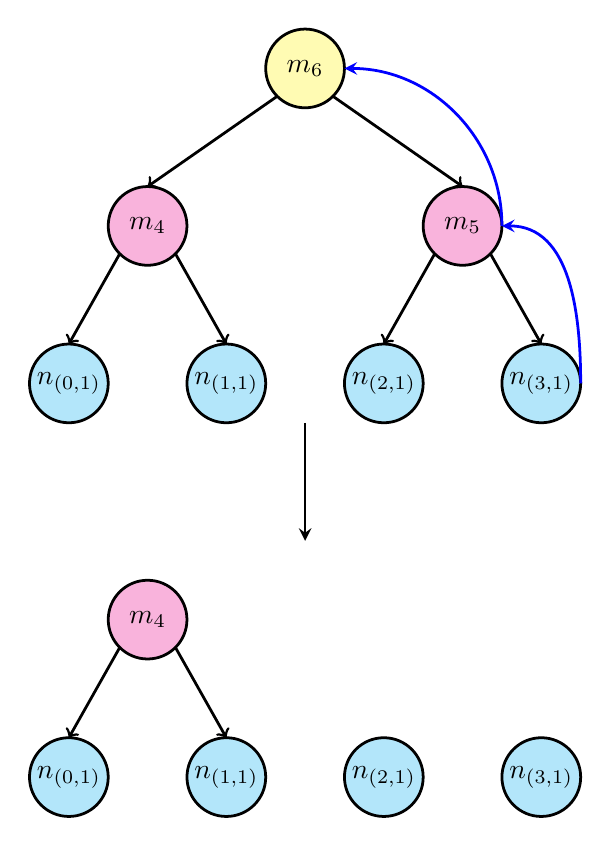
\begin{tikzpicture}[scale=0.5] % Adjust the scale factor as needed
        % Your TikZ code goes here
        \draw[line width=1pt,fill=yellow!30] (0,0) circle (1cm);
        \node at (0,0) {$m_6$};
        \draw[line width=1pt, fill=magenta!30] (-4,-4) circle (1cm);
        \node at (-4,-4) {$m_4$};
        \draw[line width=1pt, fill=magenta!30] (4,-4) circle (1cm);
        \node at (4,-4) {$m_5$};
        \draw[line width=1pt, fill=cyan!30] (-6,-8) circle (1cm);
        \node at (-6,-8) {$n_{(0,1)}$};
        \draw[line width=1pt, fill=cyan!30] (-2,-8) circle (1cm);
        \node at (-2,-8) {$n_{(1,1)}$};
        \draw[line width=1pt, fill=cyan!30] (6,-8) circle (1cm);
        \node at (6,-8) {$n_{(3,1)}$};
        \draw[line width=1pt, fill=cyan!30] (2,-8) circle (1cm);
        \node at (2,-8) {$n_{(2,1)}$};
        \draw[-> , line width=1pt] ({0 + cos(225)},{0 + sin(225)}) -- (-4,-3);
        \draw[->, line width=1pt] ({0 + cos(315)},{0 + sin(315)}) -- (4,-3);
        \draw[->, line width=1pt] ({-4 + cos(225)},{-4 + sin(225)}) -- (-6,-7);
        \draw[->, line width=1pt] ({-4 + cos(315)},{-4 + sin(315)}) -- (-2,-7);
        \draw[->, line width=1pt] ({4 + cos(225)},{-4 + sin(225)}) -- (2,-7);
        \draw[->, line width=1pt] ({4 + cos(315)},{-4 + sin(315)}) -- (6,-7);
        
        % Curved arrow
        \draw[->,>=stealth, color=blue, line width=1pt] (7, -8) to[out=90, in=0] (5, -4);
        \draw[->,>=stealth, color=blue, line width=1pt] (5, -4) to[out=90, in=0] (1, 0);
        \draw[->, >=stealth, line width=1pt] (0,-9) to (0,-12);

        \draw[line width=1pt, fill=magenta!30] (-4,-14) circle (1cm);
        \node at (-4,-14) {$m_4$};
        \draw[line width=1pt, fill=cyan!30] (-6,-18) circle (1cm);
        \node at (-6,-18) {$n_{(0,1)}$};
        \draw[line width=1pt, fill=cyan!30] (-2,-18) circle (1cm);
        \node at (-2,-18) {$n_{(1,1)}$};
        \draw[line width=1pt, fill=cyan!30] (6,-18) circle (1cm);
        \node at (6,-18) {$n_{(3,1)}$};
        \draw[line width=1pt, fill=cyan!30] (2,-18) circle (1cm);
        \node at (2,-18) {$n_{(2,1)}$};
    
        \draw[->, line width=1pt] ({-4 + cos(225)},{-14 + sin(225)}) -- (-6,-17);
        \draw[->, line width=1pt] ({-4 + cos(315)},{-14 + sin(315)}) -- (-2,-17);

    \end{tikzpicture}
    \caption{Trees and Cuts}
    \label{fig:Order_of_merging}
\end{figure}
